\chapter{强化学习}
这一部分主要是对Spinning Up教程中的内容总结。

于Model-Free RL,可以分为Policy Optimization和Q-Learning两类方法。
Policy Optimization优化方法包括:PolicyGradient、A2C/A3C、TRPO、PPO等。
Q-Learning方法包括:DQN、C51、QR-DQN、HER等。
此外还有将两种方法融合使用的,包括DDPG、TD3、SAC等。

\begin{figure}[htbp]
	\figskip 
	\centering
	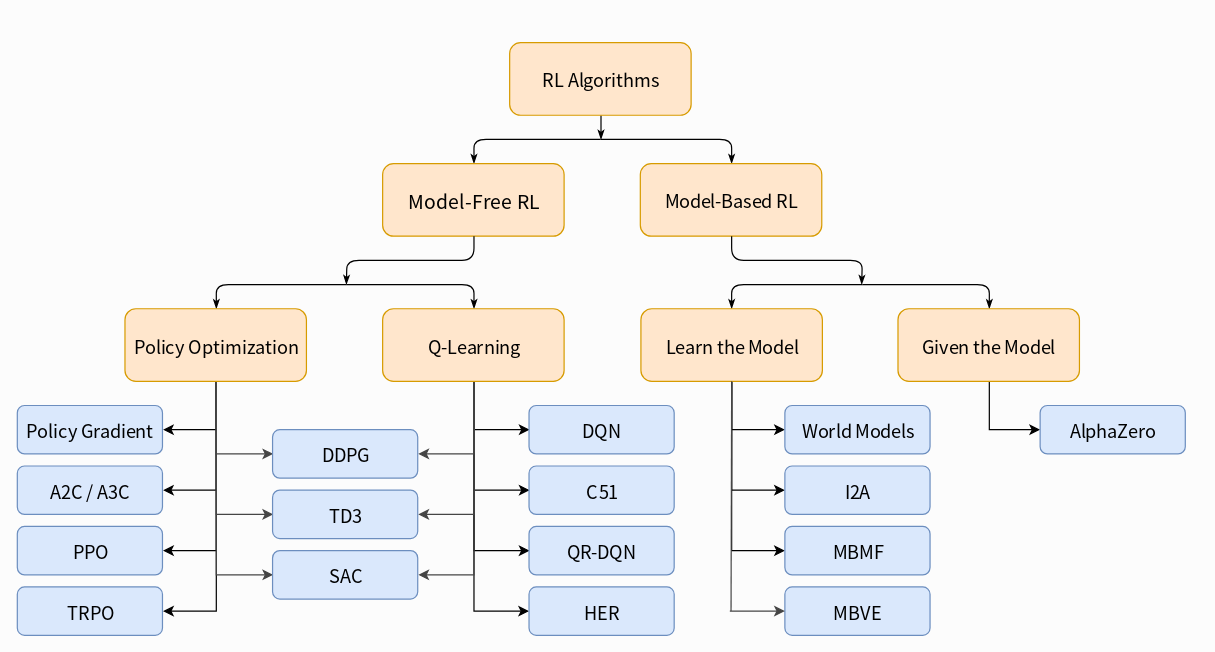
\includegraphics[width = 0.85\textwidth,trim = 0 -0 0 -0,clip]{rl-algorithms.png}	  
	\caption{\label{fig: rl} RL算法的大致分类}
\end{figure}

Policy Optimization 基本思想是直接对策略$\pi_\theta(a|s)$进行估计,
并利用目标函数$J(\pi_\theta)$最优化参数$\theta$。所以这种优化方法绝大部分都是on-policy的方式。
此外在策略优化方法的实现过程中,通常也会采用Actor-Critic的框架。
只不过一般在Policy Optimization中的Critic部分,只进行$V_\phi(s)$的估计。

Q-Learing 基本思想是用$Q_\theta(s,a)$对最优动作值函数进行估计。
通常表现为off-policy的方式。最终的策略可以表示为:
\begin{equation*}
a(s) = \arg \max_a Q_\theta(s,a)
\end{equation*}

而将两种方法结合起来的算法,就是同时估计$Q_\theta(s,a)$和$\pi_\theta(a|s)$

\section{策略优化的基础知识}
考虑随机性参数化策略$\pi_\theta$,策略的目的是将回报的期望最大化。
因此目标函数为
\begin{equation*}
    J(\pi_\theta) = \mathbb{E}_{\tau\sim\pi_\theta}[R(\tau)]
\end{equation*}

显然可以通过梯度下降的方法对策略进行优化:
\begin{equation*}
    \theta_{k+1} = \theta_k + \alpha \nabla_\theta J(\pi_\theta)|_{\theta_k}
\end{equation*}
其中$\nabla_\theta J(\pi_\theta)$称为策略梯度。
为了使用这个算法,需要显式给出策略梯度的表达式,包括两个步骤:
1)推导出策略性能的分析梯度,结果应该表示成期望的形式。
2)形成该期望值的样本估计,这个估计值可以从有限数量的样本中计算。

对于在策略$\pi_\theta$下采样获得的一条轨迹$\tau = (s_0, a_0, \cdots, s_{T+1})$,其概率为:
\begin{equation*}
    P(\tau|\theta) = \rho_0(s_0) \prod_{t=0}^{T} P(s_{t+1}|s_t, a_t)\pi_\theta(a_t|s_t)
\end{equation*}
考虑对数微分技巧:
\begin{equation*}
    \nabla_\theta P(\tau|\theta) = P(\tau|\theta)\nabla_\theta \log P(\tau|\theta)
\end{equation*}
这样轨迹的对数概率为:
\begin{equation*}
    \log P(\tau|\theta) = \log \rho_0(s_0) + \sum_{t=0}^T \left( \log P(s_{t+1}|s_t,a_t) + \log \pi_\theta (a_t|s_t) \right) 
\end{equation*}
对$\theta$求微分为:
\begin{equation*}
    \nabla_\theta \log P(\tau|\theta) = \sum_{t=0}^T \nabla_\theta \log \pi_\theta(a_t|s_t)
\end{equation*}

计算策略梯度为:
\begin{align*}
    \nabla_\theta J(\pi_\theta) &= \nabla_\theta \mathbb{E}_{\tau\sim\pi_\theta}[R(\tau)] \\
    &= \nabla_\theta \int_\tau P(\tau|\theta)R(\tau) \\
    &= \int_\tau \nabla_\theta P(\tau|\theta)R(\tau) \\
    &= \int_\tau P(\tau|\theta) \nabla_\theta \log P(\tau|\theta)R(\tau) \\
    &= \mathbb{E}_{\tau\sim\pi_\theta}\left[\nabla_\theta \log P(\tau|\theta)R(\tau)\right]
\end{align*}
代入之前的计算结果可得:
\begin{equation}{\label{eq: rl-dj}}
    \nabla_\theta J(\pi_\theta) = \mathbb{E}_{\tau\sim\pi_\theta} \left[ \sum_{t=0}^{T} \nabla_\theta \log \pi_\theta(a_t|s_t) R(\tau) \right]
\end{equation}

式(\ref{eq: rl-dj})是一个期望表达式,那么可以通过采样平均的方式进行估计。
假设我们获得了一个轨迹数据集:$\mathcal{D}=\{\tau_i\}_{i=1,\cdots,N}$,那么策略梯度就可以估计为:
\begin{equation*}
    \hat{g} = \frac{1}{|\mathcal{D}|}\sum_{\tau\in\mathcal{D}}\sum_{t=0}^T \nabla_\theta \log \pi_\theta(a_t|s_t)R(\tau)
\end{equation*}
当使用神经网络优化的方式的时候,通常定义$L(\theta) =\frac{1}{|\mathcal{D}|} \sum_{\tau\in\mathcal{D}}\sum_{t=0}^T \log \pi_\theta(a_t|s_t)R(\tau)$作为损失函数,
这样损失函数的梯度就是策略梯度。

{\hei {几个注意的地方}} 虽然上述定义了一个“损失函数”,但并不意味着它与监督学习里的损失函数具有相同的意义。
具体来说,有一下两点不同:

\noindent {\hei {1. 数据分布依赖于参数。}} 通常损失函数定义在一个固定的数据分布上,与我们待优化的参数是独立的。
但是在这里,数据需要根据最新的策略进行采样。

\noindent {\hei {2. 这里的“损失函数”无法衡量性能。}} 损失函数通常是对我们所关心的性能指标的一种估计。
在这里,我们关系期望回报$J(\pi_\theta)$,但是定义的“损失函数”并不能对其进行估计。这里“损失函数”对我们的作用只是因为,在基于当前待优化参数采样的数据集下,损失函数的梯度与性能梯度相同。
而在完成一次梯度下降之后,二者就没有什么联系了。这意味着,在给定的batch上,最小化损失函数并不能保证一定能够提高期望回报。
